\section{Results and discussion}
\subsection{Calibration}

The values that have been found for $d_{physical}$, $n_{pixels}$, $l_{pixel}$ and the corresponding error are presented in table \ref{table_pixelsize} for each objective. It was estimated that $u(n) = 4$. The images corresponding to each measurement are presented in figures \ref{fig_pixelsize_4x}, \ref{fig_pixelsize_10x} and \ref{fig_pixelsize_40x} in appendix \ref{appendix_calibration}.

\begin{table}[h!]
\centering
\captionsetup{font=small, justification = centering}
  \caption{Results of measurements of $n_{pixels}$ for the corresponding value of $d_{physical}$ for each objective. The values for $l_{pixel}$ and $u(l_{pixel})$ follow from respectfully equation \ref{eq_pixelsize} and \ref{eq_u_pixelsize}.}
\begin{tabular}{|l|l|l|l|l|}
\hline

Objective & $d_{physical} (m) \cdot 10^{-3}$ & $n_{pixels}$ & $l_{pixel}$ & $u(l_{pixel})$ \\ \hline
$4\times$ & 1 & 6.85$\cdot 10^2$ & 1.461$\cdot 10^{-6}$ & 9$\cdot 10^{-9}$\\
$10\times$ & 0.8 & 1.247$\cdot 10^3$ & 6.42$\cdot 10^{-7}$ & 2$\cdot 10^{-9}$ \\
$40\times$ & 0.2 & 1.250$\cdot 10^3$ & 1.600$\cdot 10^{-7}$ & 5$\cdot 10^{-10}$ \\ \hline
\end{tabular}

\label{table_pixelsize}
\end{table}
As expected, the accuracy for the higher magnification objectives is better. Meaning that images from an objective with a higher magnification, corresponds with a smaller value for $l_{pixel}$.\\

\subsection{Resolving power}

The photos below are the result of the process outlined in the section \ref{expmeth_calibration}. The high an low values of the line trace were manually read from the images and entered into a python script to calculating the visibility values for each magnification and spatial frequency. The result of which can be seen in figure \ref{fig:visibilities}.\\

\begin{figure}[h!]
    \centering
    \begin{minipage}{0.45\textwidth}
      \centering
      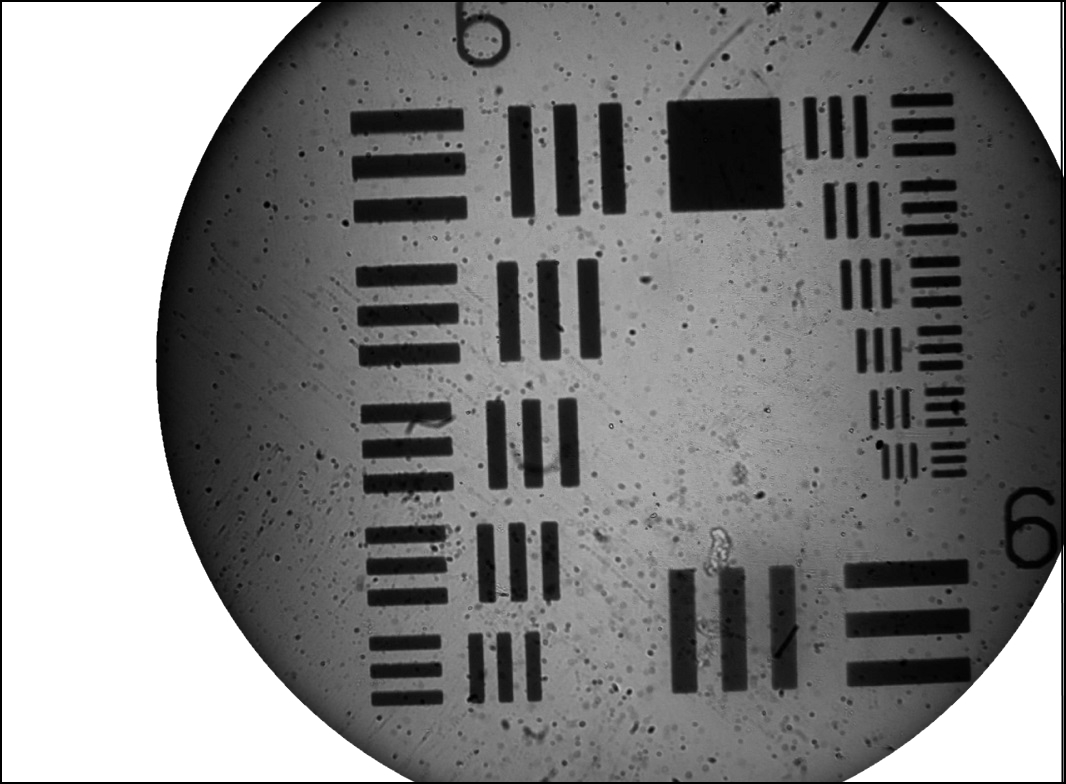
\includegraphics[width=0.7\textwidth,keepaspectratio]{afbeeldingen/process_visibility/m3_bw.jpg}
      \caption{Black and white photo.}
      \label{fig:resolution_target}
    \end{minipage}%
    \begin{minipage}{.45\textwidth}
      \centering
      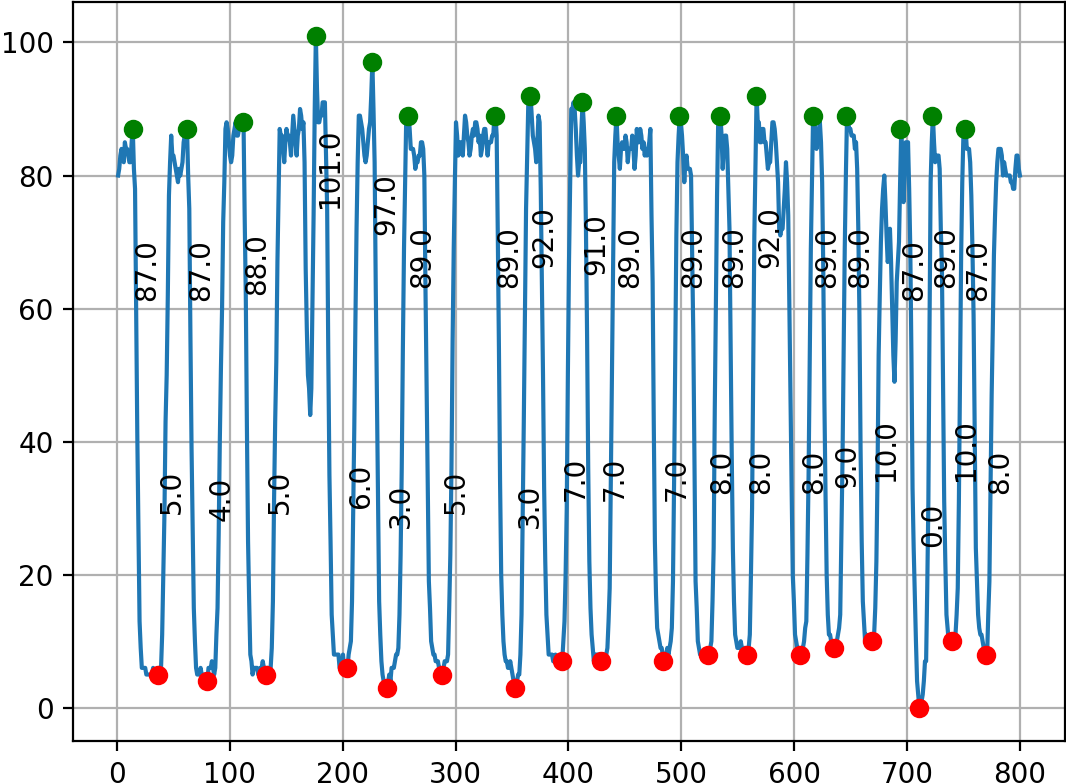
\includegraphics[width=0.7\textwidth,keepaspectratio]{afbeeldingen/process_visibility/m3_rpg_7.png}
      \caption{Linetrace of seventh group.}
      \label{fig:linetrace}
    \end{minipage}
\end{figure}


The above photos are the result of the process outlined in the section \ref{expmeth_calibration}. The high an low values of the line trace were manually read from the images and entered into a python script to calculating the visibility values for each magnification and spatial frequency. The result of which can be seen in figure \ref{fig:visibilities}.\\
The data is plotted in such a way that the highest subplot has the lowest magnification and the lowest subplot has the highest magnification. Each subplot has the dimensionless visibility number plotted on the vertical axis and the spatial frequency plotted on the horizontal axis. We chose this layout since we expect the visibility to decrease when the lines get closer together and the spatial frequency consequently increases. Note that only the vertical visibility axis of the highest sub-plot starts with a visibility of zero.\\
What we see is not surprising when we also take into account the photos in the appendix. As can be seen on these photos the $40\times$ objective has the smallest numerical aperture, therefore all three traced groups are clearly resolvable. Thus, the visibility won't drop as much for the $4\times$ objective when the spatial frequency increases.\\
Something noticeable however, is that the highest magnification plot starts of with the lowest visibility value. This has to do with the fact that this smaller aperture also catches less light, the brightest spot in its photo is evidently less bright than that of the other two apertures. This can be seen when taking a look at either the line-traces or the photos in the appendix.

\begin{figure}[h!]
    \centering
    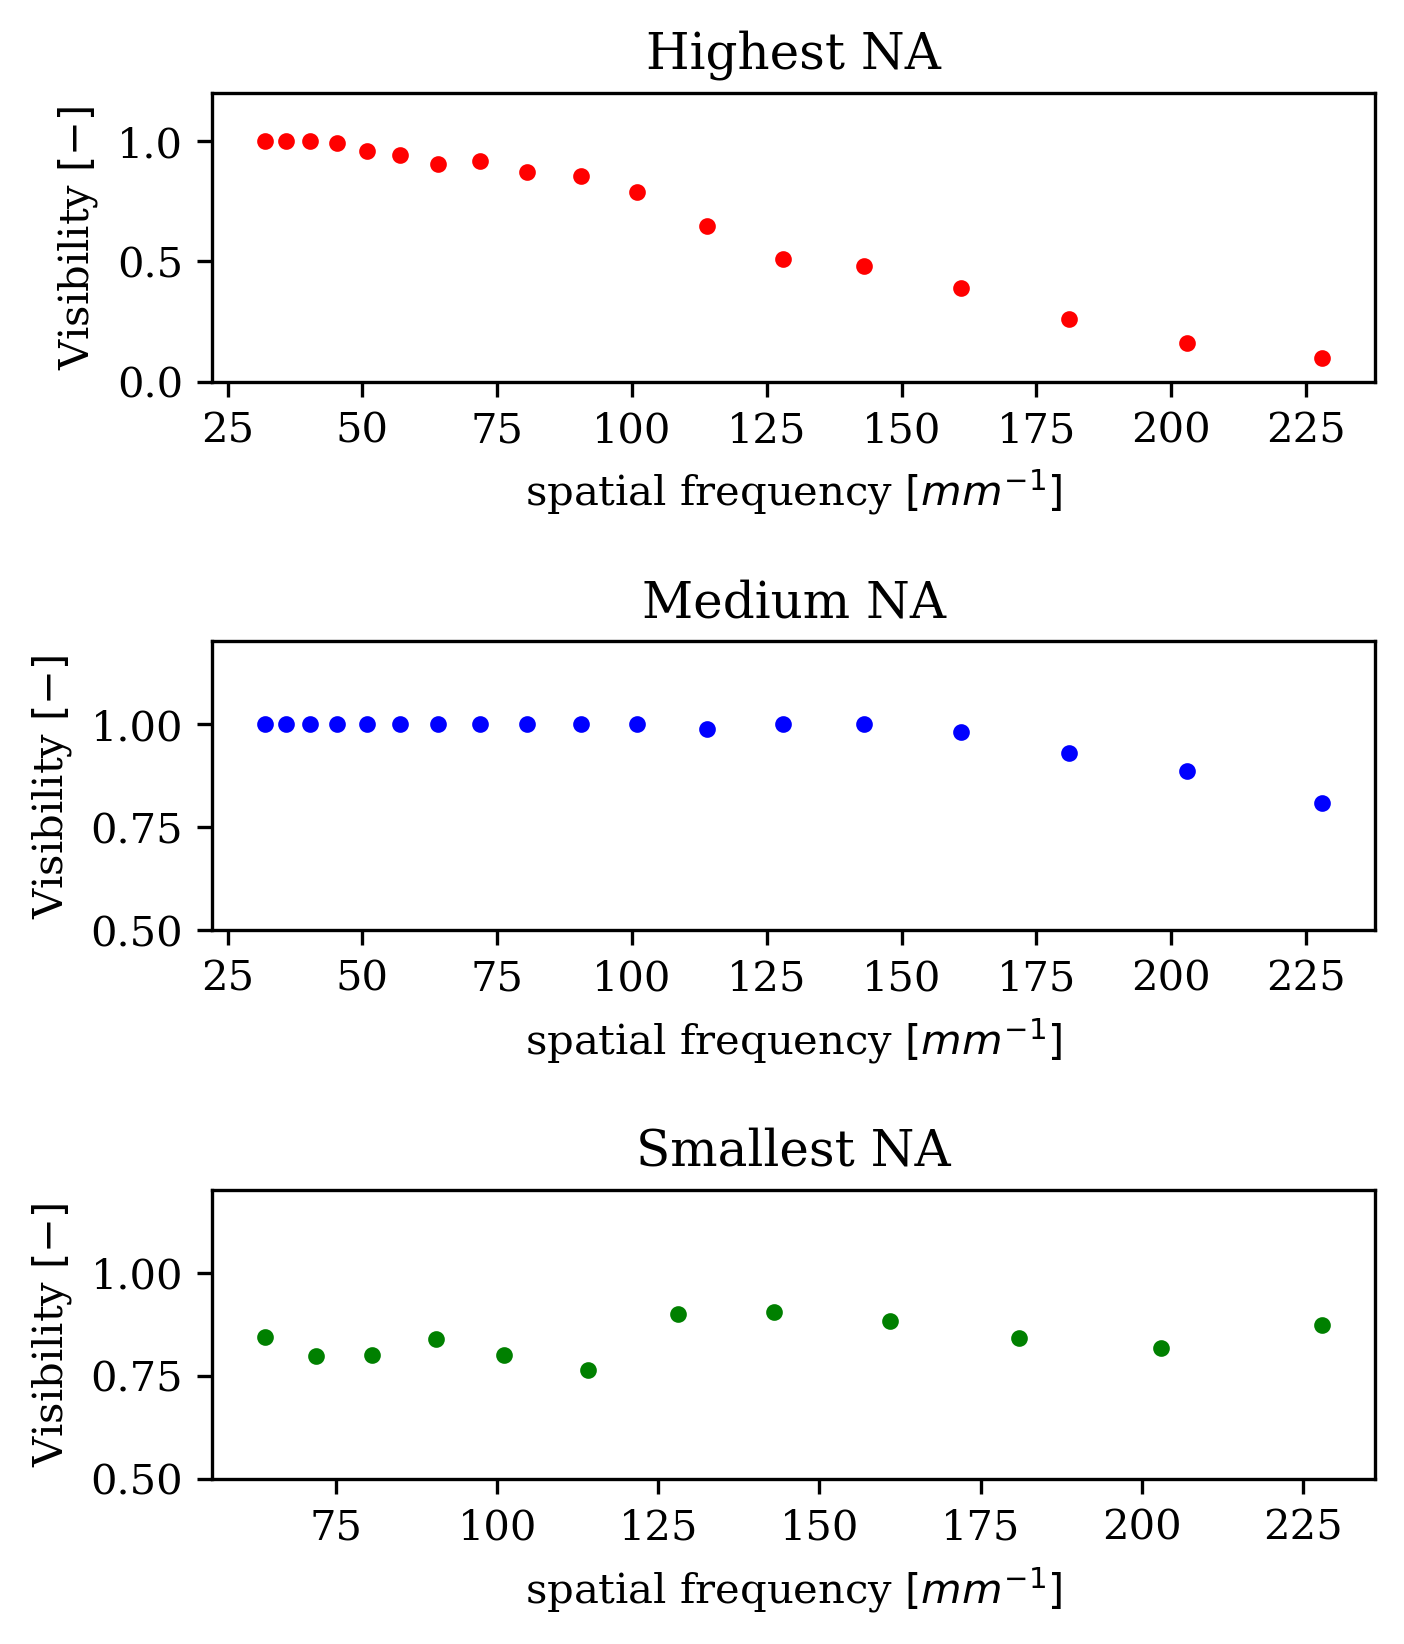
\includegraphics[width=8cm,keepaspectratio]{afbeeldingen/visibilities.png}
    \caption{Plots of the visibilities per numerical aperature.}
    \label{fig:visibilities}
\end{figure}

\subsection{Size measurements}

The values that have been found for $d_{hair}$ and $d_{gf}$ are respectively $d_{hair} = 6.57 \pm 0.08 \cdot 10^{-5} m $ and $d_{gf} =  1.26 \pm 0.01 \cdot 10^{-4} m $. The images used for the measurements are presented in \ref{appendix_size}.\\
The errors of the values for $d_{hair}$ and $d_{gf}$ are in the order of 1 \%. Furthermore, the values for $d_{hair}$ and $d_{gf}$ are of expected magnitude.

The values for $a$, $b$, $A$, the corresponding errors and the corresponding images that have been used can be found in \ref{appendix_size}. A histogram of the values for $A$ is presented in figure \ref{fig_histogram_zetmeel}.

\begin{figure}[h!]
	\centering
    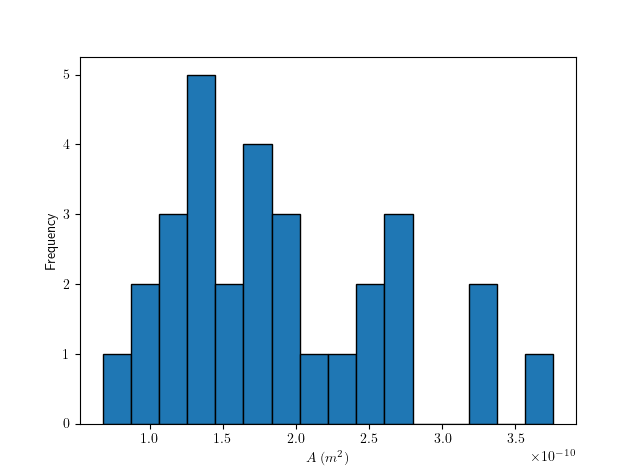
\includegraphics[width=9cm,keepaspectratio]{afbeeldingen/histogram_zetmeel.png}
    \caption{Histogram of the values of $A$ for 30 starch particles.}
    \label{fig_histogram_zetmeel}
\end{figure}

The values for $A$ are in the right order of magnitude (\cite{starch}) and have an error of under 5 \%.
The histogram shows that there is a peak for particles with a value for $A$ around $1.5 \cdot 10^{-10} \: (m^2)$. This cannot be generalised for all starch particles since only ellipse-shaped particles were taken into account. Reviewing the images that were used for the analysis (see \ref{appendix_size}) reveals that there are relatively many large starch particles that are not ellipse shaped and therefore not taken into account. Furthermore, it was only possible to get unambiguous ellipse fits for a relatively small number of particles. Most of the particles were not clearly visible or not of the right shape. Therefore, this method did not prove to be sufficient for this type of particle measurements. Other microscopy techniques, in combination with automated blob finding algorithms could possibly be of better use.

\subsection{Birefringence}

The colour planes that were taken into account for this experiment can be seen in figure \ref{fig_bf_planes} in which each Roman numeral corresponds to a colour plane. \\
The values that have been found for $f$, $\Delta l_{path}$, $D$ and the corresponding errors are presented in appendix \ref{appendix_bf}.\\
In figure \ref{fig_bf_plot}, $\Delta l_{path}$ is plotted as a function of $D$. The data point corresponding to plane $IV$, the one with the cross, was not taken into account to find $\Delta n$. The reason for this, given the distance of this data point compared to the best fit, is that it seems that an error was made during the experiment. This error could be the result of inadequate focussing on colour planes. The reason for this being the ambiguity of what details to focus on for each colour plane.\\
It follows from the orthogonal distance regression that $\Delta n = 5.3 \pm 0.2 \cdot 10^{-2}$. According to the Michel-L\'evy chart from \cite{bf_chart}, the sample could either be astrophylite, silk or piemontite.\\
The method that was used seemed to give a relatively precise outcome - only giving three possible sample materials. However, given that it is not clear why the value for colour plane $IV$ is an outsider, one could argue the validity of the outcome. \\
To find out if this experimental set-up is sufficient, the found value for $\Delta n$ should be compared to the theoretical value for the sample. This theoretical value, is however not available.

\begin{figure}[h!]

	\centering
	\begin{minipage}{.35\textwidth}
  		\centering
  		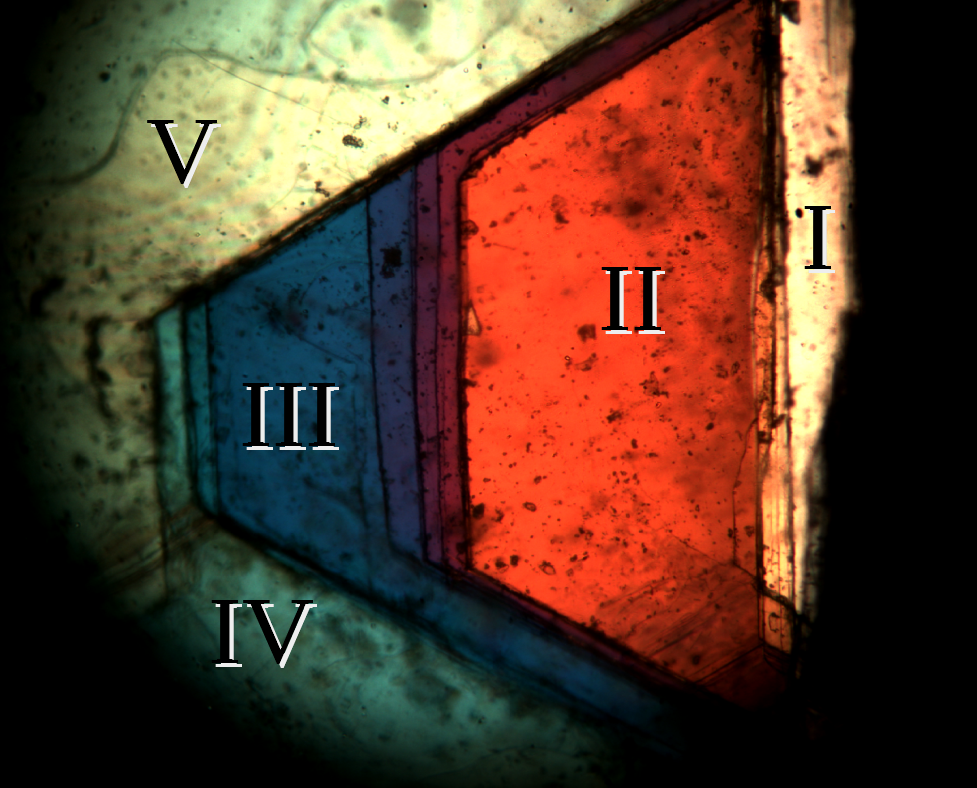
\includegraphics[width=.95\linewidth]{afbeeldingen/bf_colourplanes.png}
  		\caption{Image of a birefringent crystal in a polarizing microscope. The Roman numerals correspond to the different colour planes that were taken into account for this experiment.}
		\label{fig_bf_planes}
	\end{minipage}%
	\hfill
	\begin{minipage}{.55\textwidth}
  		\centering
  		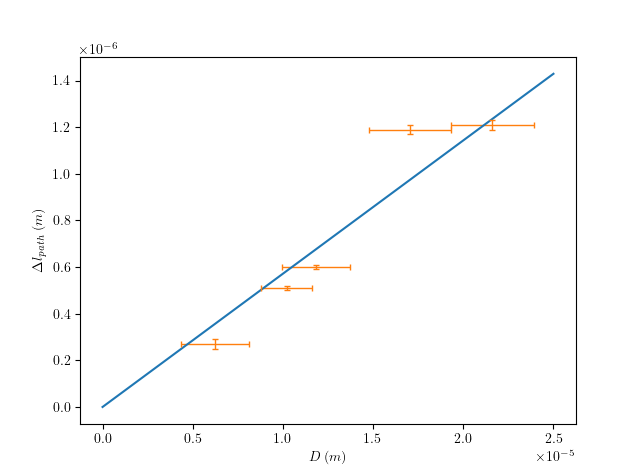
\includegraphics[width=.95\linewidth]{afbeeldingen/bf_plot.png}
		\caption{$\Delta l_{path}$ plotted as a function of $D$. The data points have errorbars in $\Delta l_{path}$ and $D$. The straight line is a best fit to the data according to an orthogonal distance regression using equation \ref{eq_bf}. The data point with the cross was not taken into account to find $\Delta n$.}
		\label{fig_bf_plot}
	\end{minipage}
\end{figure}

\newpage

\subsection{Image improvements methods}

\begin{wrapfigure}{l}{0.6\textwidth}
  \centering
  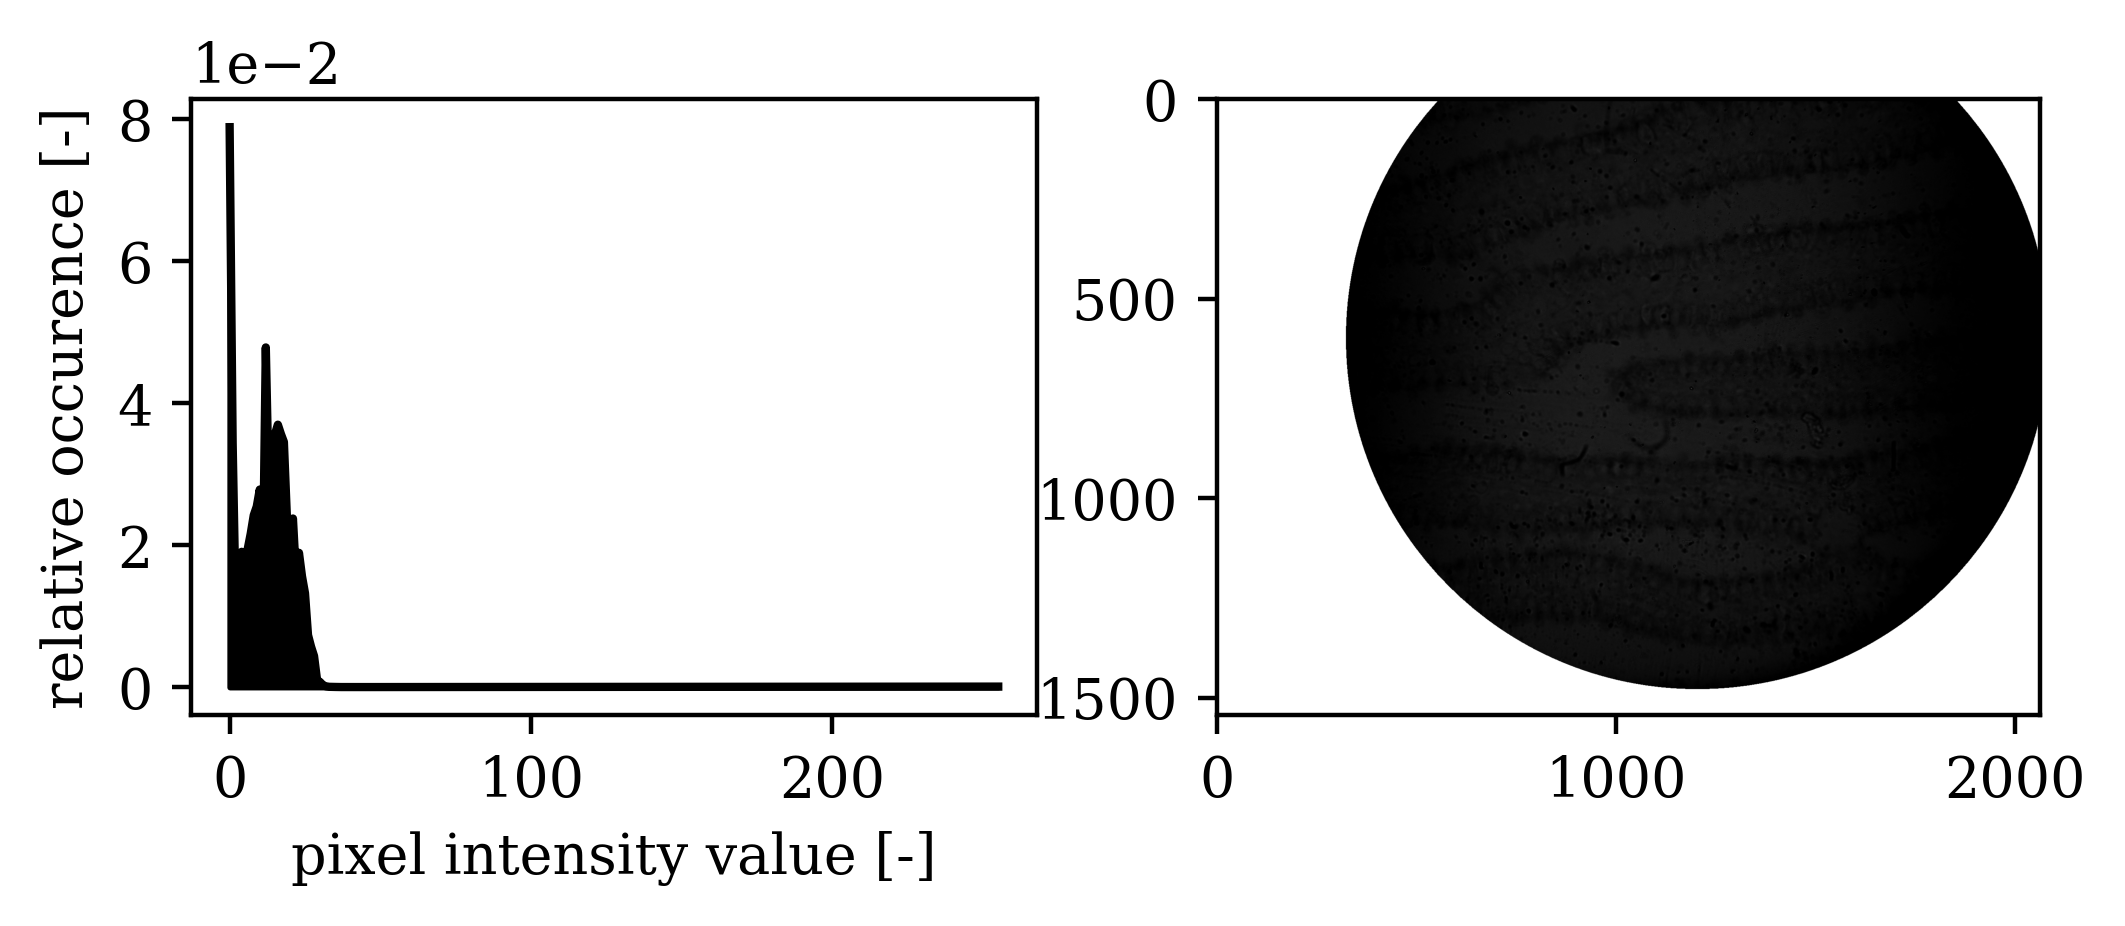
\includegraphics[width=0.55\textwidth,keepaspectratio]{afbeeldingen/Histogram_results/donkerhistogram.png}
  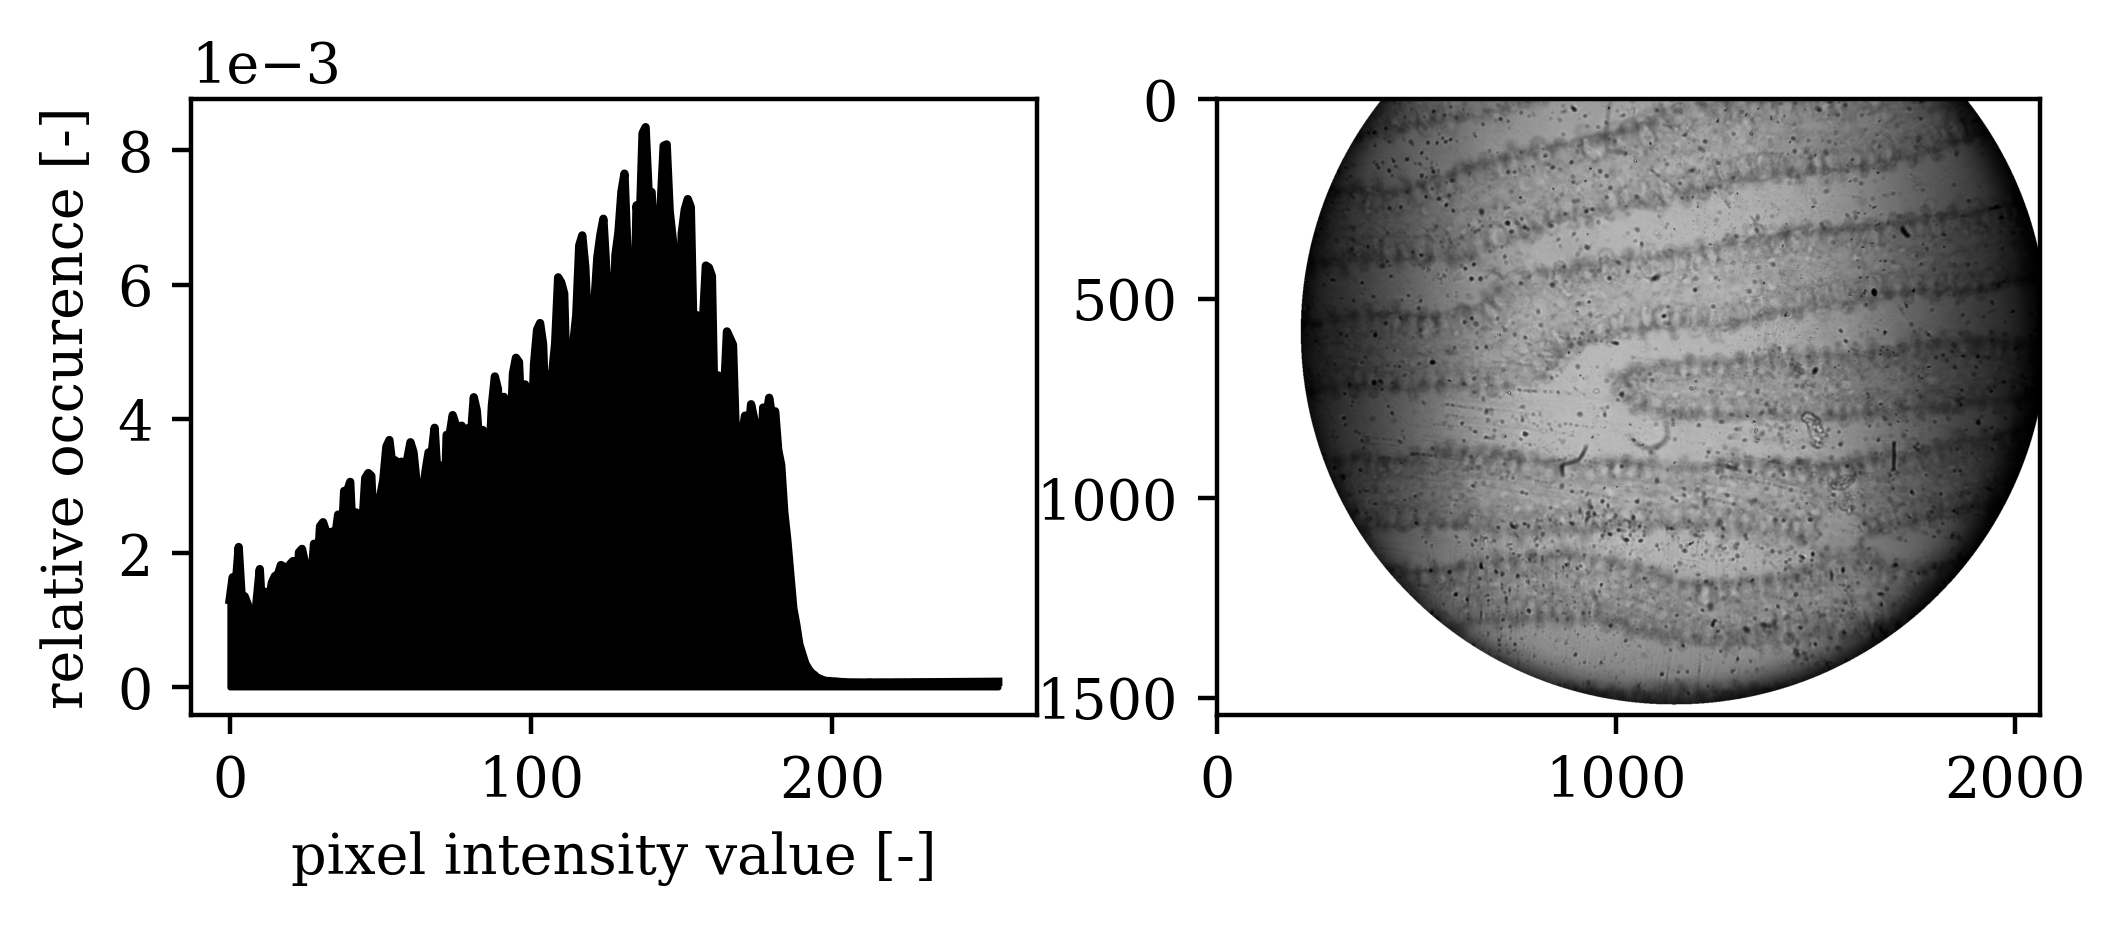
\includegraphics[width=0.55\textwidth,keepaspectratio]{afbeeldingen/Histogram_results/lichthistogram.png}
  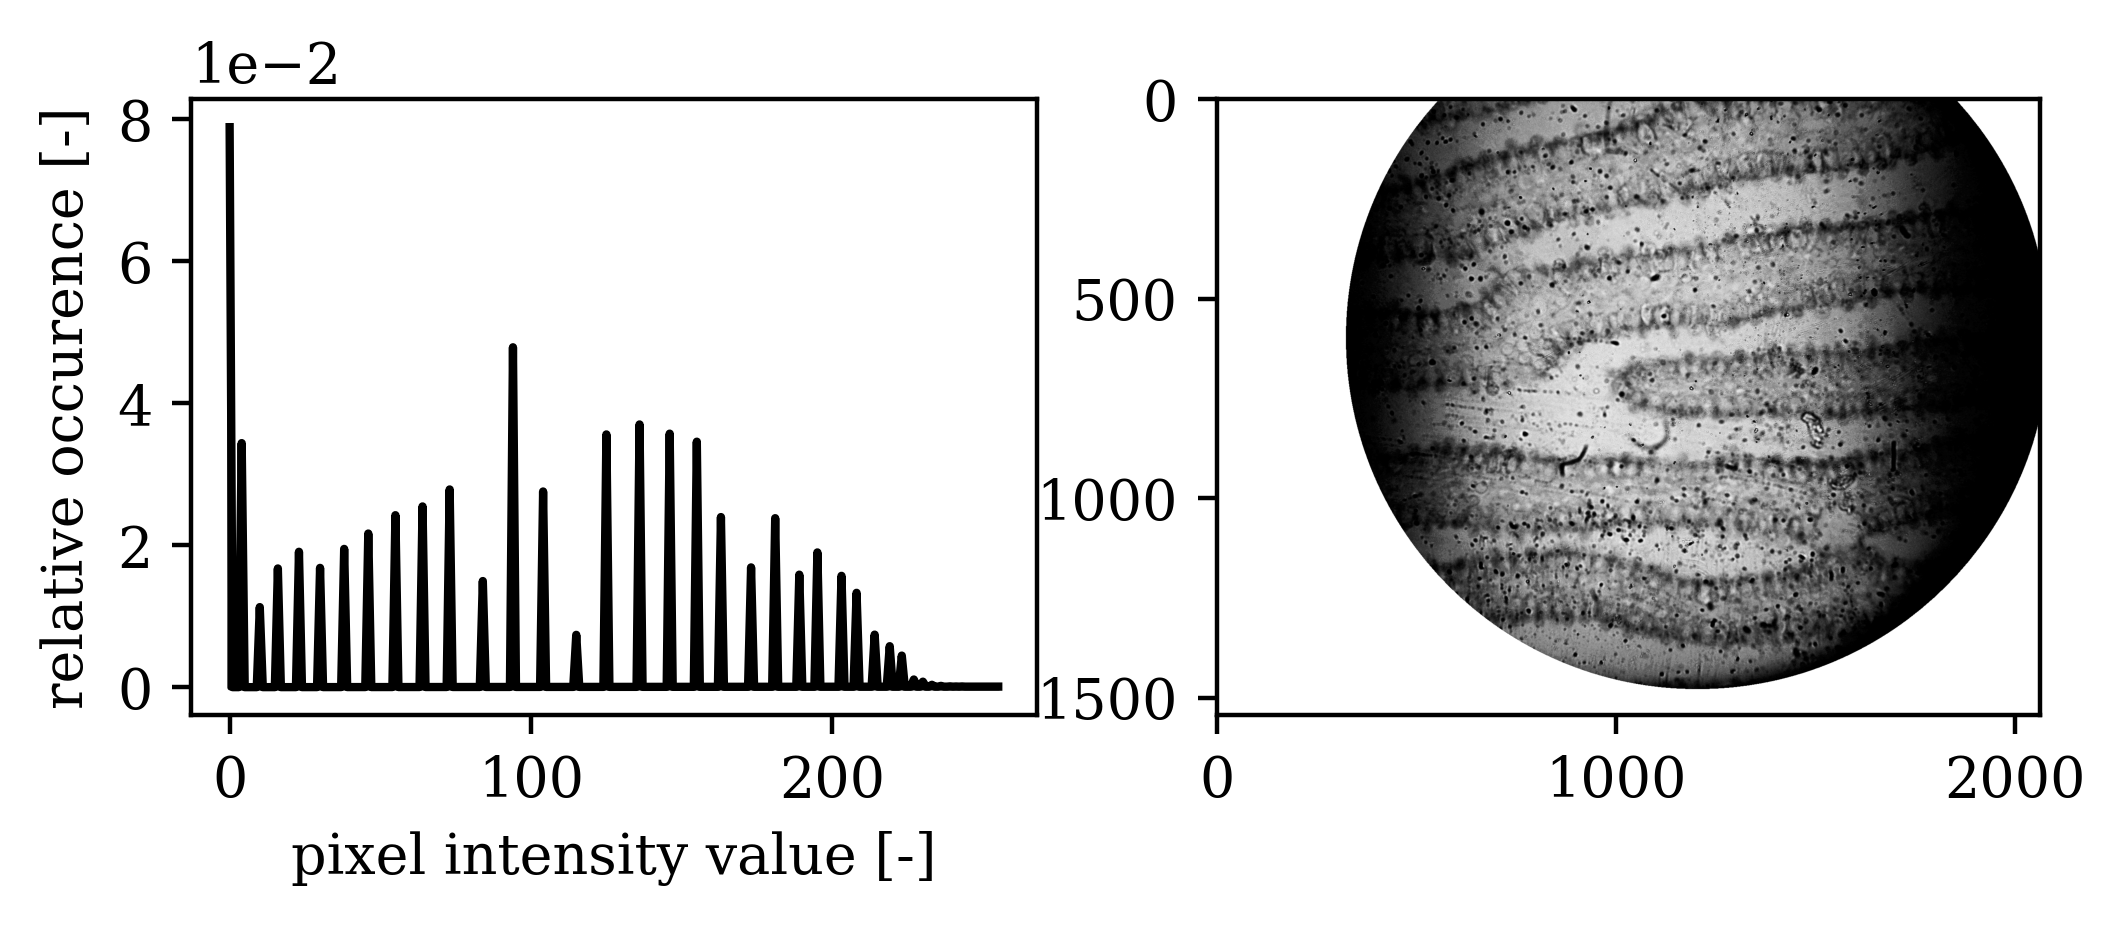
\includegraphics[width=0.55\textwidth,keepaspectratio]{afbeeldingen/Histogram_results/improved_contrast_histogram.png}
  \caption{From top to bottom: an underexposed image, an auto exposed image and the underexposed image altered by a sigmoid.}
  \label{fig:contrast_improvement}
\end{wrapfigure}

The two topmost pictures in figure \ref{fig:contrast_improvement} were taken by the same camera at different exposure settings. As can be seen the top image is clearly underexposed as the peaks of its histogram lie solely in the lowest quarter of the intensity spectrum. The second topmost image was taken at an auto-exposure setting meaning that the camera itself decides the best exposure setting. The bottommost picture contains the same information as the underexposed top image, the information however is spread over the total intensity spectrum by a sigmoid function as explained in \ref{section:imageimprovement}. The peaks of the improved image's histogram still represent the histogram of the top image.\\
Since information cannot be added to the image, the bottommost image is only better when looked at it by a person, the histogram is discontinuous meaning that there is not as much transition between two values. This is especially noticeable at the edges of the frame where the original image is so dark that there is no information to spread. Since there are only one or two intensity values the resulting shift will still only consist of two values, resulting in shifted black bars.\\
Because of the previous reason it would be safe to assume that the algorithm used could greatly improve if some sort of interpolation function is also added. This way the program would be able to try and fill in missing information.\\
\\
The original image and the image that were acquired using the $BILAT$,$CONT$ and $MORPH$ rank filters in different combinations are presented in figure \ref{fig_rank}.

\begin{figure}[h!]
    \begin{subfigure}[b]{0.5\textwidth}
        \centering
        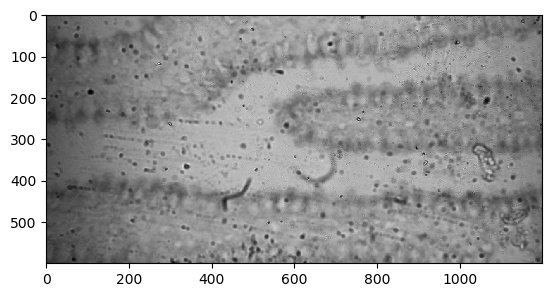
\includegraphics[width=0.8\textwidth, frame]{afbeeldingen/rank/img.png}
        \caption{Zoomed-in gray-scale image of sample.}
        \label{fig_rank_plain}
    \end{subfigure}
    \begin{subfigure}[b]{0.5\textwidth}
        \centering
        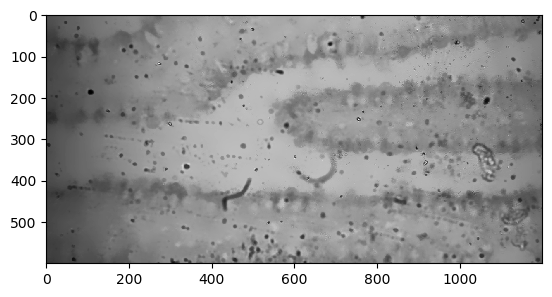
\includegraphics[width=0.8\textwidth, frame]{afbeeldingen/rank/img_bilat.png}
        \caption{Image using $BILAT$ , $r_{local}=20$ pixels.}
        \label{fig_rank_bilat}
    \end{subfigure}
\\

    \begin{subfigure}[b]{0.5\textwidth}
        \centering
        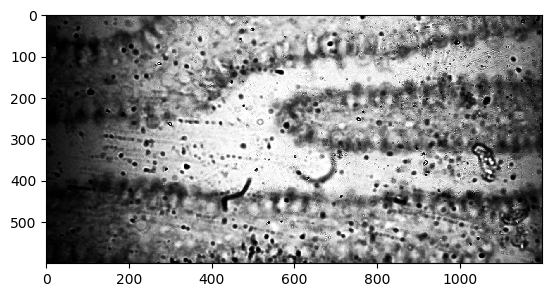
\includegraphics[width=0.8\textwidth, frame]{afbeeldingen/rank/img_cont.png}
        \caption{Image using $CONT$ , $r_{local}=5$ pixels.}
        \label{fig_rank_cont}
    \end{subfigure}
    \begin{subfigure}[b]{0.5\textwidth}
        \centering
        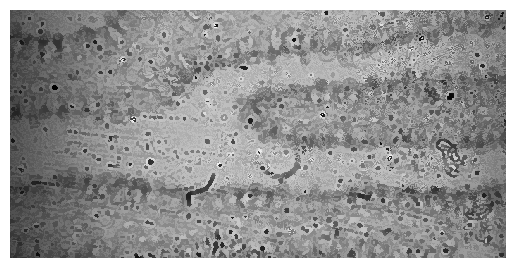
\includegraphics[width=0.8\textwidth, frame]{afbeeldingen/rank/img_morph.png}
        \caption{Image using $MORPH$, $r_{local}=5$ pixels.}
        \label{fig_rank_morph}
    \end{subfigure}
\\

     \begin{subfigure}[b]{0.5\textwidth}
        \centering
        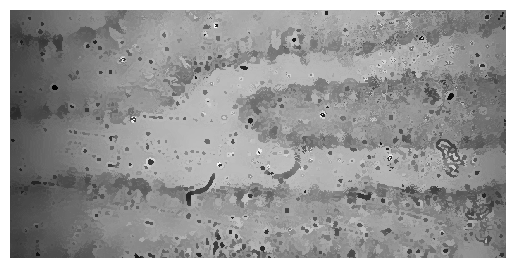
\includegraphics[width=0.8\textwidth, frame]{afbeeldingen/rank/img_morph_bilat.png}
        \caption{Image using respectively $BILAT$ and $MORPH$.}
        \label{fig_rank_morph_bilat}
    \end{subfigure}
    \begin{subfigure}[b]{0.5\textwidth}
        \centering
        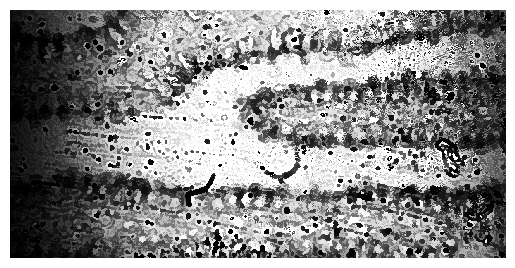
\includegraphics[width=0.8\textwidth, frame]{afbeeldingen/rank/img_morph_cont.png}
        \caption{Image using respectively $CONT$ and  $MORPH$.}
        \label{fig_rank_morph_cont}
    \end{subfigure}
\\

    \begin{subfigure}[b]{0.5\textwidth}
        \centering
        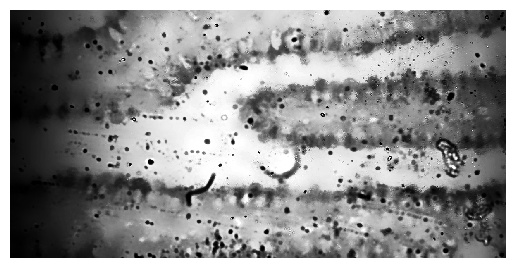
\includegraphics[width=0.8\textwidth, frame]{afbeeldingen/rank/img_cont_bilat.png}
        \vspace{3mm}
        \caption{Image using respectively $BILAT$ and $CONT$.}
        \label{fig_rank_cont_bilat}
    \end{subfigure}
    \begin{subfigure}[b]{0.5\textwidth}
        \centering
        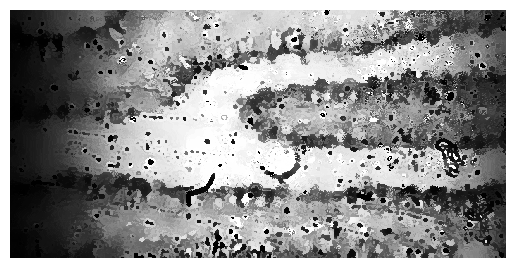
\includegraphics[width=0.8\textwidth, frame]{afbeeldingen/rank/img_morph_cont_bilat.png}
        \caption[width=1\textwidth]{Image using respectively $BILAT$, $CONT$ and $MORPH$.}
        \label{fig_rank_morph_cont_bilat}
    \end{subfigure}
\\

    \caption{Set of images using the $BILAT$,$CONT$ and $MORPH$ rank filters in different combinations}
	\label{fig_rank}
\end{figure}
\clearpage

As expected, the $BILAT$ filter filters away some of the noise. This can be seen by the reduction of small dots in figure \ref{fig_rank_bilat}. However, it also removes some of the details. \\
The $CONT$ filter improves contrast efficiently, making details more visible A downsides of the filter is, however, that it emphasizes noise and the dark edges. This causes the edges to lose quality. This could perhaps be solved by first using a high-pass filter to remove the slow darkening transition towards the edges. \\
The $MORPH$ filter makes the edges between different components in the image more clearly visible. Which could prove to be useful when doing size measurements within the image or when imposing edge detecting. What's more, it also seems to reveal more of the details. A negative artefact of the $MORPH$ filter is that it emphasizes noise. \\
Combining the filters also proves to be useful, especially combinations with the $BILAT$ filter. In this case, the noise removal and detail loss is compensated by either of the other two filters (see figure \ref{fig_rank_cont_bilat} and \ref{fig_rank_morph_bilat}). However, when many details need to be revolved, one might be better-off not using the $BILAT$ filter and accepting relatively much noise (see figure \ref{fig_rank_morph_cont}). 



